%%%%%%%%%%%%%%%%%%%%%%%%%%%%%%%%%%%%%%%%%%%%%%%%%%%%%%%%%%%%%%%%%%%%%%%%
%    INSTITUTE OF PHYSICS PUBLISHING                                   %
%                                                                      %
%   `Preparing an article for publication in an Institute of Physics   %
%    Publishing journal using LaTeX'                                   %
%                                                                      %
%    LaTeX source code `ioplau2e.tex' used to generate `author         %
%    guidelines', the documentation explaining and demonstrating use   %
%    of the Institute of Physics Publishing LaTeX preprint files       %
%    `iopart.cls, iopart12.clo and iopart10.clo'.                      %
%                                                                      %
%    `ioplau2e.tex' itself uses LaTeX with `iopart.cls'                %
%                                                                      %
%%%%%%%%%%%%%%%%%%%%%%%%%%%%%%%%%%
%
%
% First we have a character check
%
% ! exclamation mark    " double quote  
% # hash                ` opening quote (grave)
% & ampersand           ' closing quote (acute)
% $ dollar              % percent       
% ( open parenthesis    ) close paren.  
% - hyphen              = equals sign
% | vertical bar        ~ tilde         
% @ at sign             _ underscore
% { open curly brace    } close curly   
% [ open square         ] close square bracket
% + plus sign           ; semi-colon    
% * asterisk            : colon
% < open angle bracket  > close angle   
% , comma               . full stop
% ? question mark       / forward slash 
% \ backslash           ^ circumflex
%
% ABCDEFGHIJKLMNOPQRSTUVWXYZ 
% abcdefghijklmnopqrstuvwxyz 
% 1234567890
%
%%%%%%%%%%%%%%%%%%%%%%%%%%%%%%%%%%%%%%%%%%%%%%%%%%%%%%%%%%%%%%%%%%%
%
\documentclass[12pt]{iopart}
\usepackage{graphicx}
\usepackage[sf]{subfigure}
%\newcommand{\gguide}{{\it Preparing graphics for IOP journals}}
%Uncomment next line if AMS fonts required
%\usepackage{iopams}  

\begin{document}
\bibliographystyle{unsrt}

\title[Image Processing  for edge detection during GTAW]
{Image Processing and geometrical analysis for edge detection during Gaz Tungsten Metal Arc Welding}

\author{E Romero, J Chapuis, C Bordreuil, F Souli\'e, G Fras}

\address{Laboratoire de M\'ecanique et G\'enie Civil,
CC048, Place Eug\`ene Bataillon, Universit\'e Montpellier 2,
34095 Montpellier, France}
\ead{cyril.bordreuil@univ-montp2.fr}

\begin{abstract}
This paper describes some new image treatment algorithm used to 
detect profiles during arc welding process. The new algorithm 
is an aggregation of some available algorithm of image treatment,
computational geometry and graph theory. The algorithm allows to extract precise
geometrical entities as closed or open profiles that could be used for monitoring
of welding process. The algorithm  is shown to be really efficient
and could be used for real time monitoring.
\end{abstract}

%Uncomment for PACS numbers title message
%\pacs{00.00, 20.00, 42.10}
% Keywords required only for MST, PB, PMB, PM, JOA, JOB? 
%\vspace{2pc}
\noindent{\it Keywords}: Arc welding, Image treatment, weld pool,  geometrical analysis, Monitoring, 
% Uncomment for Submitted to journal title message
\submitto{\MST}
% Comment out if separate title page not required
\maketitle

\section{Introduction}

Gas Tungsten Arc Welding (GTAW), which uses a non-consumable tungsten electrode and an inert gas for arc shielding, is an extremely important arc welding process. It is commonly used for welding hard-to-weld metals such as stainless steel \cite{JUANG} and is widely use in modern and in basic industries. To achieve good weld quality in GTAW process, several weldment characteristics or objects should be sensed and controlled \cite{DOUMANIDIS}. It has been shown by Zhang et al \cite{ZHANG} that the geometry of the weld pool, in particular his shape and size, contains sufficient information about weld penetration to evaluate the weld quality. Furthermore it has been shown that the welding arc parameters to simulation and weld quality are directly relate to the weld pool geometry \cite{LU}.
Basically the weld pool object is the key in quality control to automated welding process \cite{KOVACEVIC}. 
According to this a better comprehension of the weld pool behavior presents a GTAW process, could help to improve numerical simulations and enhance welding quality in manufacturing process \cite{LIN}, \cite{WU1}. 

Many studies has been realized using visual sensing techniques to observe weld pool image \cite{BAE}. Optical sensors like high speed CCD cameras and lighting systems has been widely use in GTAW process to realize image acquisition \cite{GUANGJUN}, control process \cite{BAE} and parametric studies \cite{BALSAMO}. However, the extremely noisy environment require image processing techniques to extract useful information from visual scenes, which play a critical role in the weld pool analysis \cite{WANG}.
Nevertheless the strong interference from the arc lightning required more than standard image treatment to analyses the raw images of the welding process \cite{NORDBRUCH}. 

Previous work has shown that is possible to perform geometrical analysis in weld pools \cite{WU1}. Parameters such as weld pool contour and surface has been detected and measured using different and specifics processing images algorithms \cite{KOVACEVIC}, \cite{WU1}, \cite{SAEED}. However, to date, effectively automatic images processing of GTAW process has not been developed, possibly due to the level difficulty involved for the welding researchers \cite{WANG}.

To perform geometrical analysis in weld pool; a multipurpose C++ based library (erCv) has been developed by the Weld/Assembly group of LMGC laboratory. In the construction of this library we employed highly reliable open source libraries for image treatment, geometrical analysis, graph theory applications and image visualization.

In a first step, a reliable 2D profiles and geometrical parameters has been obtained from the weld pool using the mentioned library. This was achieved for different welding conditions: static and dynamic welding process, as well as for different current regime. Using this, a dimension and dimensionless analysis has been performed into a static and dynamic GTAW process. The intention has been to contribute to simplify futures numerical models of weld pool-arc interaction and quality process.




\section{Experimental Setup}
\label{experimental_setup}

\subsection{Multi-physics platform}
\label{multi_physics_platform}


The objective has been to perform the surface value estimation and the contour detection of the weld pool in statics and dynamics GTAW process (see \ref{fig::scheme-weld-pool-parameters}). Techniques as pool oscillations, ultrasonic sensing or infrared sensing could indirectly detect these geometric objects. However to obtain more precise measurements, Kovacevic et al. suggest direct methods as vision based techniques assisted with image processing which appears more promising \cite{KOVACEVIC}. According to this, the methods choose has been the direct image acquisition by a high speed CCD camera combined with adequate image processing techniques.


\begin{figure}
\begin{center}
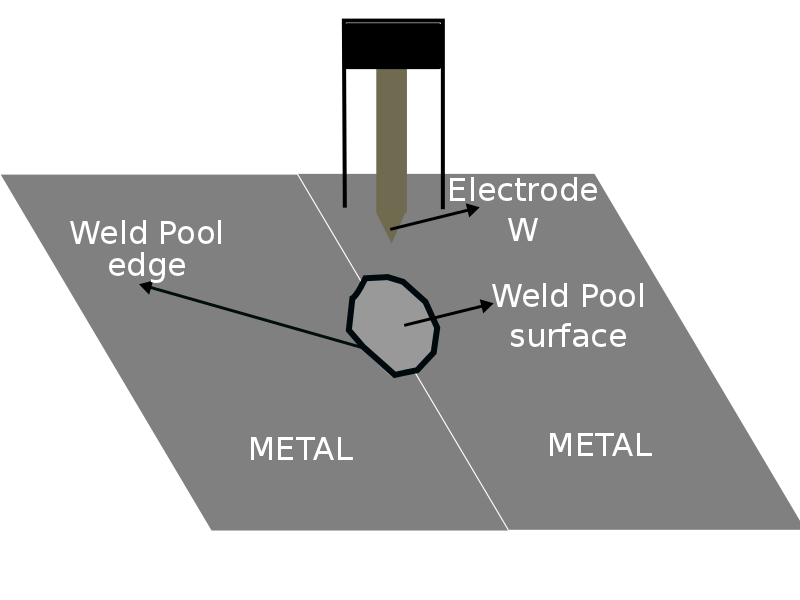
\includegraphics[width=7cm,height=4cm]{scheme-weld-pool-parameters.png}
\caption{{\small Overview schematics of welding objects in a GTAW process}}
\label{fig::scheme-weld-pool-parameters}
\end{center}
\end{figure}


To perform the geometrical analyses of weld pool, it has been necessary correlate the weld pool images with the welding parameters. Then different signals of control and measurements have had to be synchronized and recorded \cite{CHAPUIS}. This require accurate, reliable and synchronizes systems due to the high amount of data and highly noisy environment (electromagnetic noise and arc light radiation). 

In order to this, a platform has been developed at the laboratory to perform multi-physics measures in arc welding process 
%(see figure \ref{fig::schema-platform}). 
The platform was conceive with an automatically procedure to synchronize, to acquire, to manage and to exploit large flow of multi-physical experimental data (up to 2 Go per test). This characteristic allows synchronizing (in time) the current and voltage signals with the acquired images.

%\begin{figure}
%\begin{center}
%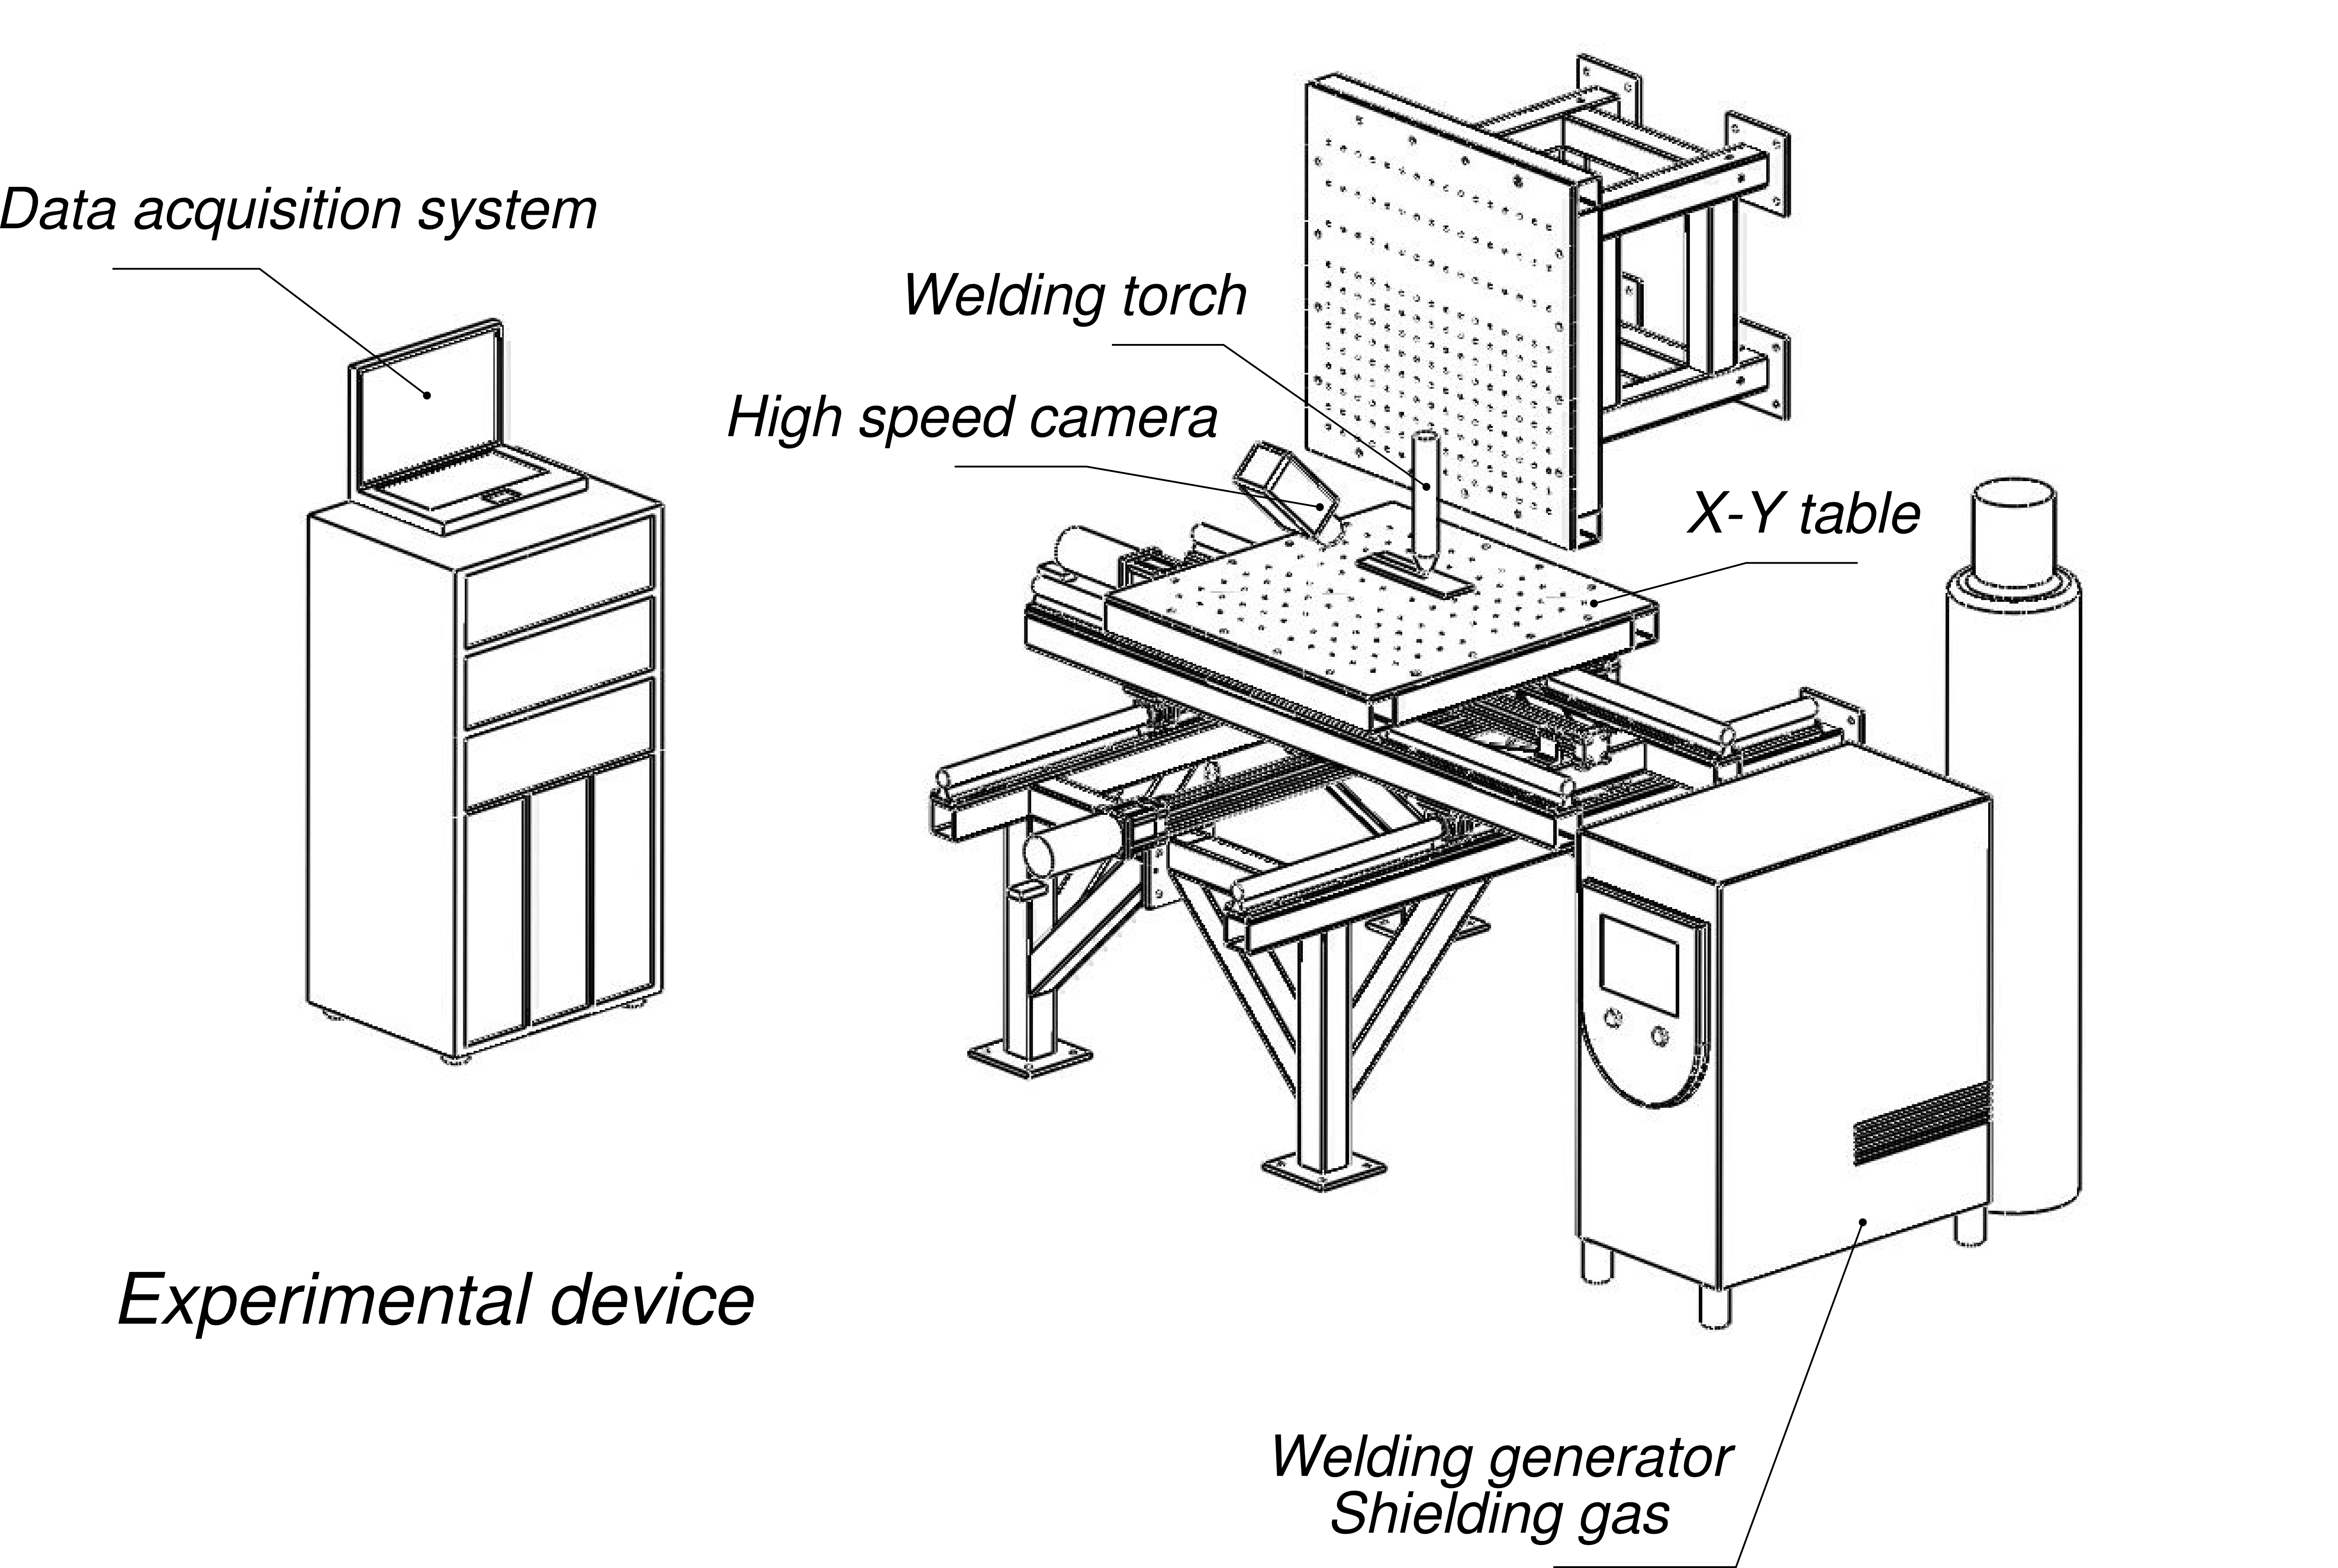
\includegraphics[width=7cm,height=4cm]{schema-platform.png}
%\caption{{\small Experimental platform and specific device}}
%\label{fig::schema-platform}
%\end{center}
%\end{figure}

The general data (without the image) analyzes and processing has been performed using a multi-physics measures database; a numerical open source library developed by the laboratory. 



\subsection{ Image acquisition setup}
\label{image_acquisition_setup}

Using a similar technique employed by Kovacevic et al. \cite{KOVACEVIC}, the GTAW static process has been recorded by the specular reflection optical method. A $650\ nm$ laser diode has been used to light the weld process from an estimate angle of $35\ degree$. The laser beam width ($ ??? $) has been enough to guarantee a homogeneous illumination of the welding process. The laser projects, by reflection, an image of the welding objects (weld pool and surrounding metal substrate) to the other side of the welding place. In this place and aligned with the optical path of the reflected laser beam, a Phantom V5.0 high speed camera has been placed in order to record the images of the process (see figure \ref{fig::scheme-adquisition-setup}). 

\begin{figure}
\begin{center}
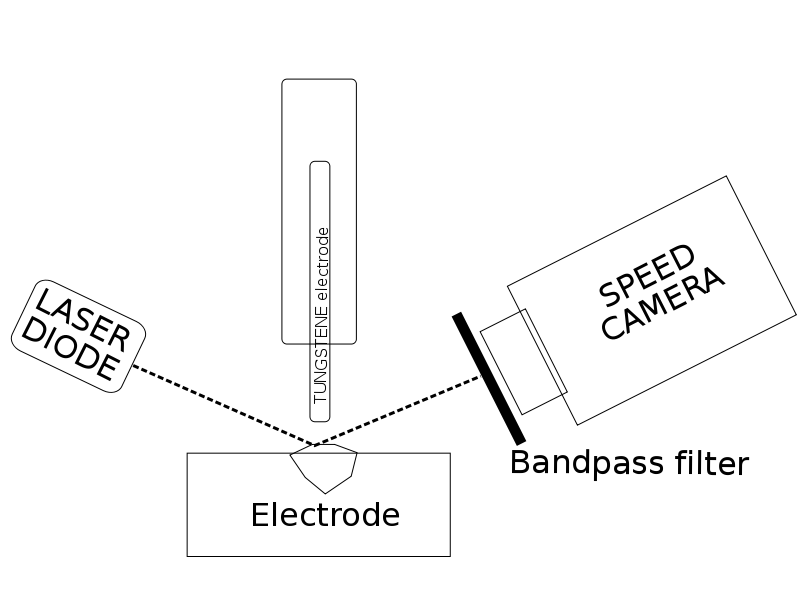
\includegraphics[width=7cm,height=4cm]{scheme-adquisition-setup.png}
\caption{{\small Experimental setup to detect weld pool edges in GTAW process}}
\label{fig::scheme-adquisition-setup}
\end{center}
\end{figure}

To enhance the image contrast of the weld objects inside the electric discharge, the intensity rate between the arc light and the laser diode must have been reduced. In order to this a $650\ \pm 10\ nm$ band pass filter, which correspond to the laser diode wavelength, has been placed in front of the camera lens to attenuate the arc light. Nevertheless, the raw images remain highly noisy due to the arc light intensity and disturbed by the non-homogeneous reflections over the dynamic and non-flat weld pool surface. 


% ON CONTINUE ICI
\subsection{ Welding condition}
\label{ welding_conditions}



\subsection{Image treatment library}
\label{image_treatment_library}

In order to solve the mentioned limitations of the image acquisition technique and to perform geometrical analysis above the weld elements, a multipurpose image processing library has been developed and is currently use at the laboratory. This library, called erCv, can manage different kinds of image acquisition (optical setup). And therefore is able to perform edge detection and geometrical analysis in different welding elements such as macro drop, droplets and weld pool. The library is implemented in an oriented object C++ language. Then, erCv is a scalable and portable library able to perform real time contour detection. The library is implemented in C++ with some bindings in python, making it relatively convivial to use for non-programmers. To manage the edge detection during welding process, four processing modules compose the library (see figure \ref{fig::scheme-structure-library}):  
\begin{description}
\item[Image Treatment:] Due to weld process conditions such arc lightening, heat and electrodes positions; the raw image registered by CCD camera are not calibrated and present light inhomogeneities and noise. In order to obtain the real shape and size of the welding elements, this module includes calibration algorithms. To detect the welding elements contours it is necessary to improve the welding images. This module has the pre-processing treatments for noise reduction and image enhancement.
Then to start the edges detection process, this module includes processing algorithms as segmentation by samples comparator, watershed transformation, filters edge detectors and histogram based methods.  Most of the functionality comes from \cite{OPENCV}.
\item[Geometrical Treatment and Analysis:] This module convert the isolated points of the edges pixels into connected segments to conclude the edge detection process, completing and in some cases extrapolating the welding elements edge. It is also responsible to compute the geometrical data of welding elements such weld pool surface and metal transfer drop volumes. 
  This module uses a full geometry algorithm library\cite{CGAL}, which include different algorithms such as triangulations and mesh generation, alpha shape and convex hull generation and polygonal structures.
\item[Graph Theories:] To compute the geometrical data of welding elements it is necessary to extract the profile contour of the welding element from the image; this require some criteria such as continuity, length or closing condition. Applying these criteria, this module use graph algorithms to identify and to select the welding element contour. This module is composed by connected segments, estimates minimal cut, determine largest chain segments and others algorithms. 
   The algorithm of \cite{BOOSTGRAPH} are used.
\item[Visualization:] This module is a set of functions used to execute, show and/or register the different steps at the image processing.
\end{description}

\begin{figure}
\begin{center}
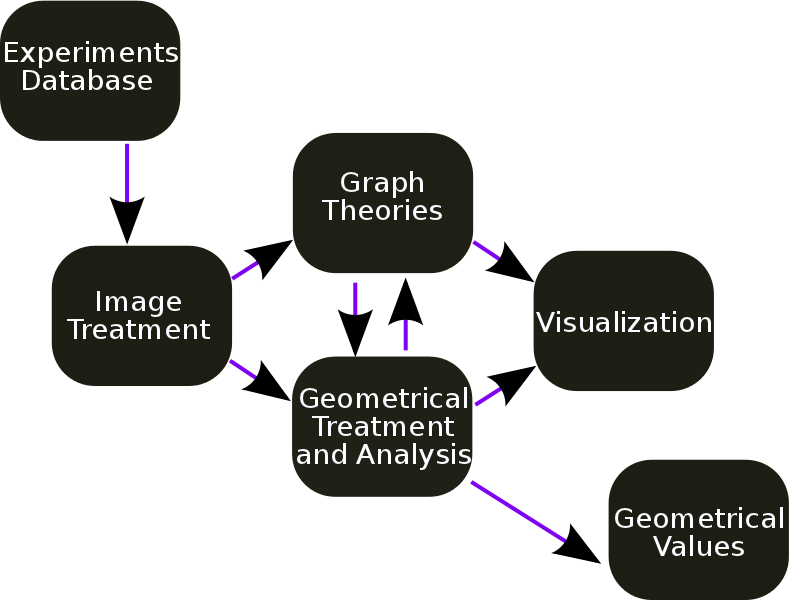
\includegraphics[width=10cm]{scheme-structure-library.png}
\caption{{\small Flow diagram of erCv library composition}}
\label{fig::scheme-structure-library}
\end{center}
\end{figure}

The originality of the library comes from the aggregation and complementarities of the different numerical tools.
The main difficulty is to find algorithms with good parameters all along the process.


      
      



\section{Image processing tools} 
\label{ image_processing_tools}

Some definitions and a brief description of the general principles used in image processing are required to better understand how erCv perform the geometrical analysis of the weld pool, despite the noisy environment.
 

\subsection{Image treatment basics}
\subsubsection{Some definitions}
\label{some_definitions}

A numerical grey image can be described as a 3D surface divided by a grid mesh in the $(X,Y)$ plane. Each square represents a pixel and the relief surface in $Z$ axis the grey level. 
A strong relief change at the image, or high gradient of grey values in the plane $(X,Y)$, are perceived by human eyes as light changes and can be interpreted as objects edges. 

Sometimes, a regular relief patrons or regular grayness level variation can be distinguished. The human eyes can perceive these patrons as texture and interpret the space between different textures zones as edges.
There exist a large spectrum of algorithms to perform image treatment, in particular for edges detection.
Most of them can be classified in the way that they operate above the image pixels and grayness level.


\subsubsection{Filters}
\label{filters}

The filters are algorithms which operates as mathematical functions $f$ above the 
$X$, $Y$ or both axis of the image ($Z = f(X,Y)$,  
$f(X)$ or $f(Y)$)  modifying his grayness value or $Z$ component. 
Different kind of filters can be mentioned as median, Gaussian, impulse, adaptive and others. The impulse filters, such as Canny, are widely uses to perform edge detection \cite{COCQUEREZ}. These filters have an impulse response to most of the important grayness level gradient in the image; this allows the filter a better edges localization (see figure \ref{fig::image-explanation-filter}). 
For this reason, Canny filter has been extensively used into the library to detect welding elements edges. 
However, the Canny filter is sensible to noise or secondary grayness gradients in the image and, in consequence, it have some difficulties to define closed surface.



\subsubsection{Snake and level set}
\label{snake_and_level_set}
 
The curve propagation is a popular technique in image analysis for object extraction, object tracking, edge detection and others (see figure 
\ref{fig::image-explanation-snake}). The central idea behind this approach is to make evolve a curve towards the lowest potential of a cost function. 
However at each stage of the curve evolution, the potential at each curve point has to be computed. A lot of point (better curve resolution) take a lot computing time, and therefore are not yet apply to real time detection or relatively high frequency automatic image processing. For this reason snake algorithms has not been used into the erCv library.


\subsubsection{Segmentation}
\label{segmentation}

Let $B$ an image and let $R_{i}$ an arbitrary region of $B$ such:

\begin{eqnarray}
B = \bigcup_{i}R_{i}\ \forall i \in \{0, \mbox{numbers of regions in B}\} \\
\mbox{with}\ R_{i} \neq \emptyset \\
\mbox{and}\  R_{i}\bigcap R_{j} = \emptyset\ \forall i, j\ \mbox{with}\ i \neq j\ 
\label{equation-segmentation}
\end{eqnarray}

Perform a $B$ segmentation means perform an image treatment which generate a $B$ partition in $R_{i}$ regions. 
Each region is a connected set of pixels with common properties (intensity, texture and others) \cite{COCQUEREZ}.
 The partition is generated by operations or comparisons methods between regions. Generally, this treatment offers a good edge detection if the elements and his surrounding area have different textures (see figure \ref{fig::image-explanation-segmentation}). Note that different regions can belong to the same partition, therefore the surface is not always connected and, in consequence, the edges of the interest regions are not always closed.

\begin{figure}[h!]
\begin{center}    
\subfigure[Weld pool image in static GTAW process]{\label{fig::image-explanation-patron}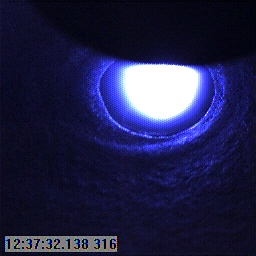
\includegraphics[width=3.5cm,height=3.5cm]{image-explanation-patron.png}}
\subfigure[Canny filter treatment]{\label{fig::image-explanation-filter}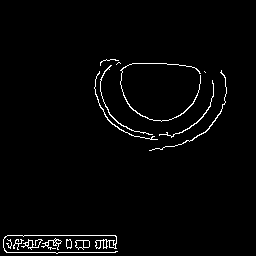
\includegraphics[width=3.5cm,height=3.5cm]{image-explanation-filter.png}}\\
\subfigure[Snake treatment]{\label{fig::image-explanation-snake}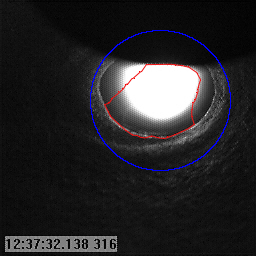
\includegraphics[width=3.5cm,height=3.5cm]{image-explanation-snake.png}}
\subfigure[Segmentation image by 2 cluster sample comparison]{\label{fig::image-explanation-segmentation}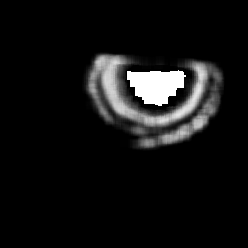
\includegraphics[width=3.5cm,height=3.5cm]{image-explanation-segmentation.png}}
\end{center}
\caption{{\small Representative samples of the different methods technique to perform image processing}}
\label{fig::image-explanation}
\end{figure}


% On s ARRETE LA



\section{ Applying image processing}
\label{ applying_image_processing}

\subsection{ First Image Adjustment}
\label{first_image_features}


It has been mentioned in section \ref{filters}, that most of the filter type algorithm (including canny filter) operates as function over the image grayness levels. Moreover, the segmentation processing requires less computing time over 1-channels image than over 3-channels image. In order to allow to use filters algorithm and to do more efficient the image processing, a function has been include into the treatment module to convert the color image of the weld pool into a grayness level image (see image \ref{fig::image-weldpool-greyness}).


\begin{figure}[h!]
\begin{center}    
\subfigure[Raw image]{\label{fig::image-weldpool-original}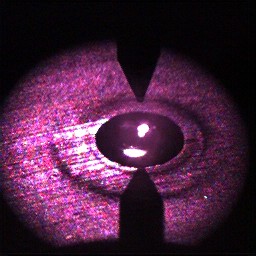
\includegraphics[width=3.5cm,height=3.5cm]{image-weldpool-original.png}}
\subfigure[Grey level image]{\label{fig::image-weldpool-greyness}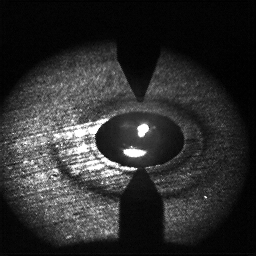
\includegraphics[width=3.5cm,height=3.5cm]{image-weldpool-greyness.png}}\\
\end{center}
\caption{{\small Raw recording image}}
\label{image-correction}
\end{figure}


\subsection{ Image Preprocessing}
\label{image-preprocessing}


The idea is to recognize the weld pool into the raw image, extract a well define weld pool contour and therefore calculate his 2D surface area. Several approaches have been developed and can be used to obtain the weld pool contour: the edge detection techniques \cite{WU2} as level set or impulse filters, the Hough transforms \cite{OLSON} or the geometrical weld pool division \cite{KOVACEVIC}; nevertheless the most common approach is the image segmentation \cite{WANG}. 

Previous works \cite{WU2}, \cite{KOVACEVIC} has shown that thanks to the optical acquisition method (specular reflection), the mirror like surface of the weld pool reflect a smoothness dark surface to the camera while the solid metal surface reflect an irregular grayness level surface. As like as the eyes recognize the texture in a object surface and$/$or image, this particularity in the grayness level distribution at the image could be interpreted as roughness variations or different textures zones \cite{MATERKA}. And this propriety can be used to perform images segmentation dividing the image between the roughness zone and the smoothness dark zone (like the weld pool area, see figures \ref{fig::image-weldpool-greyness}). 

This technique know as texture analysis is an image processing technique widely used in biomedicine, satellite recognition, quality control and others fields requiring image processing. There exist different approaches to texture analysis, each one using their own image analysis methods: Structural, statistical, model based and transform methods \cite{MATERKA}. The structural method requires complex logical analysis, while the transform and model based methods require the identification and analysis of deterministic properties in the grayness level distributions \cite{MATERKA}. Finally the statistical method compares intuitively to what human eyes recognize: surfaces with an irregular grayness level distribution or roughness, which matches to what has been observed in the recorded images (see images \ref{fig::image-weldpool-greyness}).

However the low intensity contrast between the weld pool and the surrounding surface (solid metal, induce error in the texture analysis. It is due to the radiation from the pool, as well as the impurities or oxides present in both surfaces (see figure \ref{fig::image-weldpool-greyness}). The impurities outside the weld pool could be interpreted as dark smoothness zone like the weld pool and not as roughness zone, while the edge of impurities and light reflections into the weld pool could be interpreted as roughness zone. Therefore isolate the weld pool require more than a simply approach using one of the existing techniques. Indeed perform 2D contour require an effective techniques combination to correct the light reflection distortions and impurities, isolate the weld pool from the image and extract his contour.



\subsubsection{Impurities and light reflects correction on the weld pool}
\label{impurities-and-reflex-correction}

%Before isolate the weld pool from the image, the arc reflects and the impurities over the 
%weld pool have to be reduced. 

Note that the impurities and the high intensities reflection appear as white blobs (high gray values set of pixels) into the dark weld pool (low gray values set of pixel, see figure \ref{fig::image-weldpool-greyness}). An algorithm able to detect the ��white�� blobs into the weld pool and correct its has been developed and included into the image treatment module of erCv. The algorithm use the same principia used by the red eye detections and corrections algorithm \cite{GAUBATZ}.

The white blob correction algorithm uses three threshold values to fix the blob selection criteria: $g_{upper}$ to define the minimal gray level of the ��white blob��, $g_{lower}$ to define the maximal gray level of the weld pool and $s_{max}$ to define the blob maximum pixel sizes. 

Call $B$ an arbitrary ��white�� blob set, $\partial B$ his boundary and $size(B)$ his size in pixels numbers. Call $(x, y)$ a pixel coordinates at the image and $gray\_level( x, y)$ the pixel associate grayness level.

\begin{eqnarray*}
( x, y)\ \in\ B\ \mbox{if} \\
gray\_ level( x, y) > g_{upper} \\
\mbox{Then}\ B\ \mbox{is in the weld pool if} \\
gray\_ level( x, y)\ \leq\ g_{lower}\ \forall\ (x,y) \in\ \partial B \\ 
\mbox{and if}\ size(B)\ <\ s_{max}
\end{eqnarray*}

If $B$ is into the weld pool, the gray value at each pixel $(x,y)$ inside $B$ is replaced by the gray average value of the gray value pixels of $\partial B$ (see equation \ref{equation-grayness-recouvrement}). Then the ��white�� blob is replaced by a low average grayness level surface, similar to the rest of the weld pool grayness level. 

\begin{equation}
gray\_level( x, y)\ =\ \frac{gray\_level( x, y_{\partial B}) + gray\_level( x_{\partial B}, y) }{ 2}
\label{equation-grayness-recouvrement}
\end{equation}

Using this algorithm, most of the impurities and the arc light reflections into the weld pool have been corrected (see figure \ref{fig::image-correction-weldpool-whiteblob}).
	



\subsection{ First Image Adjustment}
\label{first_image_features}

Before to describes an effective procedure using filtering or segmentation algorithms from the erCv library, the image view angle imposed by the image acquisition procedure, have had to be modified. 

As shown in section \ref{image_acquisition_setup}, the camera records a specular reflection of the welding process. Therefore the image of the welding objects is not orthogonal to the optical axes of the camera. In order to correct the image perspective, a function has been included in the image treatment module. A control image (small chessboard image with known real dimensions) is recorded at the weld pool place (see figure \ref{fig::image-correction-chessboard-raw}). An algorithm recognizes the chessboard corners and builds a transformation matrix between the chessboard recorded image and the original digital image (see figures \ref{fig::image-correction-chessboard-draw}). This transformation matrix allows the algorithms to correct the weld pool image perspective (see figures \ref{fig::image-correction-weldpool-whiteblob}, \ref{fig::image-correction-weldpool-perspective}) Finally, to calibrate the image dimension (in pixels) to the real objects dimension (in millimeters), a conversion scale is applied with the real dimensions of chessboard control image $conv = 1\ mm/ 20\ pixels$. 

\begin{figure}[h!]
\begin{center}    
\subfigure[Chessboard control image]{\label{fig::image-correction-chessboard-raw}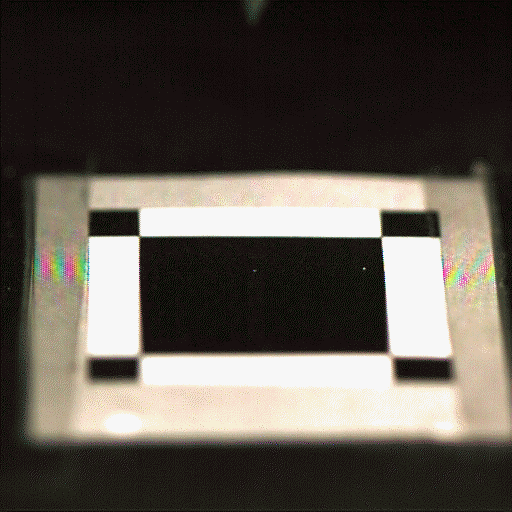
\includegraphics[width=3.5cm,height=3.5cm]{image-correction-chessboard-raw.png}}
\subfigure[Chessboard original digital image]{\label{fig::image-correction-chessboard-draw}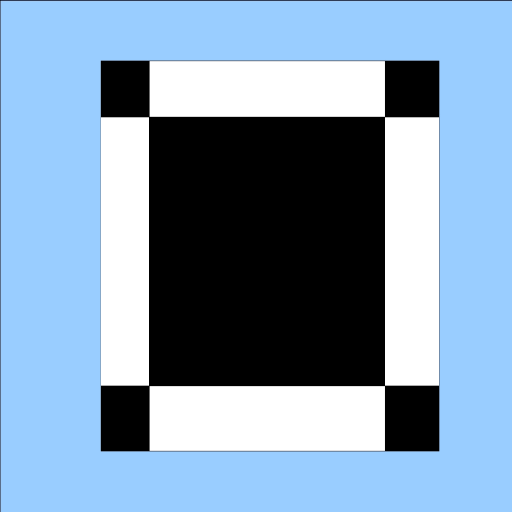
\includegraphics[width=3.5cm,height=3.5cm]{image-correction-chessboard-draw.png}}\\
\subfigure[White blob corrected image]{\label{fig::image-correction-weldpool-whiteblob}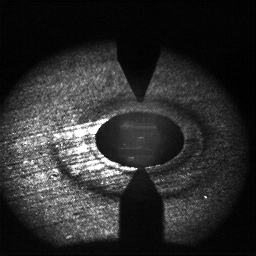
\includegraphics[width=3.5cm,height=3.5cm]{image-weldpool-whiteblob.png}}
\subfigure[Perspective corrected image ]{\label{fig::image-correction-weldpool-perspective}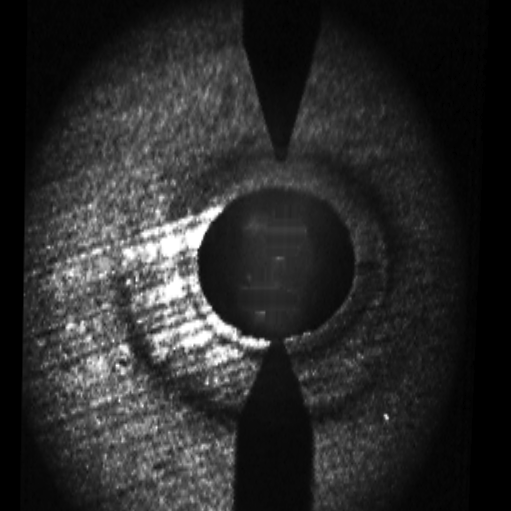
\includegraphics[width=3.5cm,height=3.5cm]{image-weldpool-perspective.png}}\\
\end{center}
\caption{{\small Perspective image correction patrons}}
\label{image-correction}
\end{figure}




\subsubsection{ Impurities and light reflects corrections surrounding the weld pool}
\label{impurities-and-light-reflects-corrections-surroinding-the-weld-pool}

As mentioned the presence of some oxides impurities into the solid metal surface, closer to the weld pool edge, rest a mayor problem to image segmentation. A combination of filtering and segmentation techniques has been applied to reduce the brightness points and dark zones due to impurities presence into the roughness zone.
 
First, an impulse response filter to grayness level gradient is applied (Canny filter). This filter converts the grayness level images into images composed only by white segments (the edges profiles). Adjusting the filter parameters to maximum gradient detection, the canny filter read the irregular grayness level distribution as multiple grayness level gradients. Then the roughness surfaces are converted into irregular and dense zone with white segments distributions and the smoothness zone are converted into almost zero level zones (black zones as the weld pool). The impurities appear as small black zones surrounded by numerous white segments into the roughness zone or solid metal surface (see image \ref{fig::image-weldpool-canny1}). 

The idea is replace the roughness zone by a more homogeneous white surface recovering the small black zones. A dilate filter have been applied (twice) to enhance the white segments up to small white surfaces reducing the small black zones corresponding to the impurities into the solid metal surface (see figure \ref{fig::image-weldpool-dilate}). This filter operate taking the maximum value over a $3\times 3$ pixel neighborhood. A smooth classical filter (blur) has been used to smooth the ��white surfaces edges��. This filter replaces the values of squares of $5\times 5$ pixels by their average values. The small black zones into the biggest white surface appears diffused due to the smoothness effect over the edges (see figure \ref{fig::image-weldpool-smooth}). The same effect is observed into the biggest black zone (weld pool), where the small white surfaces become highly diffused. Then, a median filter types have been used to enhance the image by gray values region, and homogenized the surfaces. This filter compute the grayness median value over $5\times 5$ pixels region. The image is enhance in his black (weld pool) and white (solid metal) regions (see image \ref{fig::image-weldpool-median}), resulting in a more homogeneous white and black surfaces. 


\subsubsection{Completing the image segmentation}
\label{completing-the-image-segmentation}

In order to recognize and to isolate the weld pool element, which now appears as a central black surface into the image (see image \ref{fig::image-weldpool-median}),  a segmentation statistical algorithm has been applied. A small region of interest (ROI) is defined into the weld pool. Then the algorithm scans the image surface by regions of equal ROI size. The algorithm find similarities to the ROI using a normalize correlation method.  The gray values of the resulting regions are adjusted depending their level of correlation with the ROI; $0$ gray value means non correlation at all while $255$ gray value means that it is the same surface. Note that the weld pool became the big central white region (see image \ref{fig::image-weldpool-segmentation})

A threshold of type binary have been applied to enhance the edge of the white surfaces, converting the image into a binary white and black regions follows the criteria:

$
\begin{array}{l}
gray\_ level\_ threshold(x,y) = 
\end{array}
\left\{ 
\begin{array}{lcr}
    0 & if & gray\_ level\_ original(x,y)\ <\ 200 \\
255 & if & gray\_ level\_ original(x,y)\ \geq\ 200 
\end{array}
\right\} $

Where $gray\_level\_original(x,y)$ is the gray value of a image pixel before the threshold and $gray\_level\_threshold$ is the gray value assign to the pixel after the threshold (see figure \ref{fig::image-weldpool-threshold}.

Finally a Canny filter has been applied to extract the principal edges presents in the image. Note that for a binary image all edges are principal, therefore Canny detect all edges presents into the image (see figure \ref{fig::image-weldpool-canny2}).



\begin{figure}[h!]
\begin{center}    
%\subfigure[Raw image]{\label{fig::image-weldpool-original}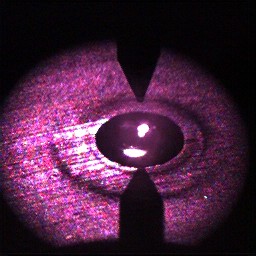
\includegraphics[width=3.5cm,height=3.5cm]{image-weldpool-original.png}}
%\subfigure[Grey level image]{\label{fig::image-weldpool-greyness}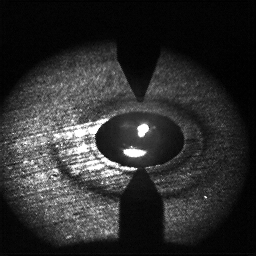
\includegraphics[width=3.5cm,height=3.5cm]{image-weldpool-greyness.png}}\\
%\subfigure[White blob corrected image]{\label{fig::image-weldpool-whitblob}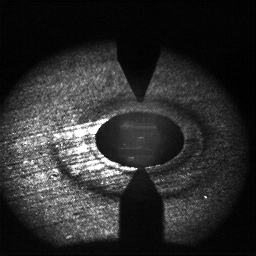
\includegraphics[width=3.5cm,height=3.5cm]{image-weldpool-whiteblob.png}}
%\subfigure[Perspective corrected image ]{\label{fig::image-weldpool-perspective}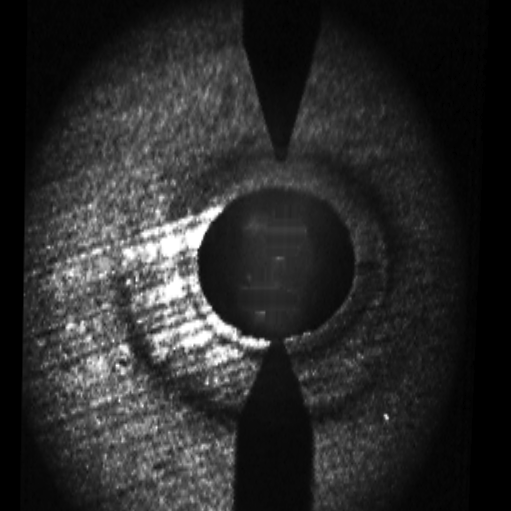
\includegraphics[width=3.5cm,height=3.5cm]{image-weldpool-perspective.png}}\\
\subfigure[First canny filter application]{\label{fig::image-weldpool-canny1}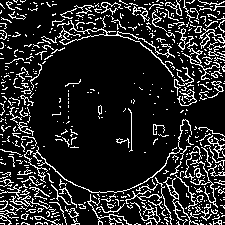
\includegraphics[width=3.5cm,height=3.5cm]{image-weldpool-canny1.png}}
\subfigure[Dilate application]{\label{fig::image-weldpool-dilate}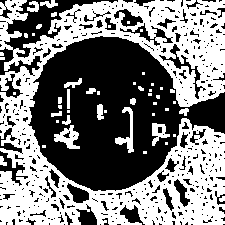
\includegraphics[width=3.5cm,height=3.5cm]{image-weldpool-dilate.png}}\\
\subfigure[Smooth application]{\label{fig::image-weldpool-smooth}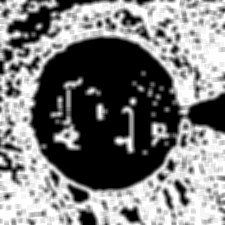
\includegraphics[width=3.5cm,height=3.5cm]{image-weldpool-smooth.png}}
\subfigure[Median application]{\label{fig::image-weldpool-median}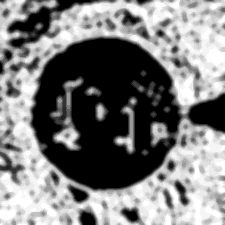
\includegraphics[width=3.5cm,height=3.5cm]{image-weldpool-median.png}}\\
\subfigure[Segmentation algorithm]{\label{fig::image-weldpool-segmentation}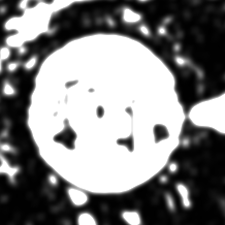
\includegraphics[width=3.5cm,height=3.5cm]{image-weldpool-segmentation.png}}
\subfigure[Threshold application]{\label{fig::image-weldpool-threshold}
\includegraphics[width=3.5cm,height=3.5cm]{image-weldpool-threshold.png}}\\
\subfigure[Second canny filter application]{\label{fig::image-weldpool-canny2}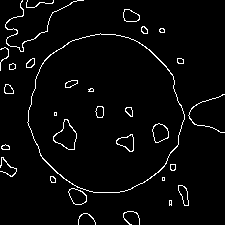
\includegraphics[width=3.5cm,height=3.5cm]{image-weldpool-canny2.png}}
\end{center}
\caption{{\small Perspective image correction samples}}
\label{image-correction}
\end{figure}


\subsection{Edge extraction}
\label{edge_extraction}

Despite the performance achieved by the image processing, the canny filter generates many edges or strings into the image. These strings are composed by white points and are interpreted by the algorithms as individual�s points. In order to automate the weld pool edge extraction process, geometrical and graph algorithms have been used to connect the points belonging to the weld pool border, convert it into connected segments and compute the area surrounded by the segments.

Note that the weld pool appears as the biggest closer string into the figure \ref{fig::image-weldpool-canny2}. The idea is to build segments around the string and take the longest closer set of segments. 

Give $S$ the set of points into the space image. The segments could be built between wherever two points of $S$. However to fulfill the strings with segments, only the points placed together could define a segment. To choose the correct point of $S$ a Delaunay Triangulation is made over $S$ \cite{CGAL}. Each point of $S$ is a vertex of a triangle and then each potential segment is an edge of a triangle. The Delaunay triangulations guarantees a unique solution with minimal internal angles for each triangle, which means minimal length sides to the triangles \cite{BERG}. Give $\beta$ the string surrounding the external hull of the Delaunay triangulation of $S$. An alpha shape algorithm uses a  $\alpha\ \in\ N$ parameter, or square radius of a test circle, to travel from outside $\beta$ to inside the triangulation. The circle has to go through the triangles sides without touching the vertices. Give $n$ the number of triangles sides of the triangulation and $l_{i}$ with $i\ \in\ {1,n}$ the length of each side, if $\sqrt{\alpha}\ >\ l_{i}$ with $i\ \in\ {1,n}$ , a segment is marked between the respective vertices or points. At the end of the process, a set of segments knows as $\alpha$-shape has been created. Note if $\sqrt{\alpha} > l_{i}\ \forall\ i$, the circle can not go inside $\beta$, then $\alpha$-shape is $\beta$ \cite{CGAL}. If $\sqrt{\alpha}\ <\  l_{i}\ \forall\ i$ the circle go through every side in the triangulation, then  no segment  is created and $\alpha$-shape became $S$. The points that compound the weld pool borders are all contact neighbors. Then $\alpha\ =\ 1$ is sufficient to create a segment set around the droplet (see figure \ref{fig::image-weldpool-alphashape}).

A graph algorithm connects these segments and finds the longest closer segment. The longer closer segment corresponds to the weld pool perimeter (see figure \ref{fig::image-weldpool-graphconected}).




\subsection{Geometrical Analysis}
\label{geometrical_analize}


\section{ Results}
\label{results}


\subsubsection{Discussions}
\label{discussion}




\section{ Conclusions}
\label{conclusions}



\section*{Acknowledgment}
The authors want to thanks the Agence National pour la Recherche (ANR) which grants this research
under the ANR-JCJC038 young scientist contract. 
\section*{References}
$ $
%\bibliographystyle{unsrt}
\bibliography{paper_bain_drop}

%\section*{References}
%\begin{thebibliography}{10}
%\bibitem{book1} Goosens M, Rahtz S and Mittelbach F 1997 {\it The \LaTeX\ Graphics Companion\/} 
%(Reading, MA: Addison-Wesley)
%\bibitem{eps} Reckdahl K 1997 {\it Using Imported Graphics in \LaTeX\ } (search CTAN for the file `epslatex.pdf')

% \cite{BALSAMO}
%\cite{WANG}
%\cite{CHO}
%\cite{LIN}
% \cite{ZHANG4}
%\cite{BAE}
%\cite{NORDBRUCH}
%\bibitem{CGAL} http://www.cgal.org 
%\cite{ChapuisThesis}
%\cite{WU1}
%\cite{SEED}
% \cite{COCQUEREZ}
% \cite{OPENCV}
% \cite{GEOMETRICAL}
% \cite{white}
%\end{thebibliography}
\end{document}


